% Course report prepared with the Springer Nature article class, version 3.1
% (December 2024), and a Tribhuvan University project-report front matter.
\documentclass[pdflatex,sn-vancouver-num]{sn-jnl}

\usepackage[T1]{fontenc}
\usepackage{graphicx}
\usepackage{amsmath,amssymb,amsfonts}
\usepackage{newtxtext,newtxmath}
\usepackage{booktabs}
\usepackage{xcolor}
\usepackage{placeins}

\hypersetup{
    pdftitle={Comparative Evaluation of Five Machine Learning Classifiers for Diabetes Outcome Classification},
    pdfauthor={Sandesh Poudel, Sankalpa Gautam, and Tilak Thapa},
    hidelinks
}

\raggedbottom

% Match the project-report convention used in the supplied layout reference.
\renewcommand{\sectionfont}{\normalfont\fontsize{14}{16}\selectfont\bfseries\centering}
\makeatletter
\renewcommand{\ps@plain}{%
    \let\@mkboth\@gobbletwo
    \let\@oddhead\@empty
    \let\@evenhead\@empty
    \def\@oddfoot{\vbox to 18pt{\vfill\reset@font\rmfamily\hfil\thepage\hfil}}%
    \let\@evenfoot\@oddfoot
}
\makeatother

\newcommand{\reportabstract}{We compared five classifiers on the binary \texttt{Outcome} field of the Pima Indians Diabetes dataset: a custom $k$-nearest neighbours classifier, a decision tree, a calibrated support vector machine, Gaussian Naive Bayes, and a multi-layer perceptron. The dataset contains 768 records; a stratified split assigned 614 to training and held out 154 for testing. Under the preprocessing rule used in this project, zero entries for glucose, blood pressure, skin thickness, insulin, and body mass index were treated as missing. We fitted median imputation and standard scaling only on the training data before applying both transformations to the test data. The decision tree recorded the highest accuracy (78.57\%), sensitivity (68.52\%), F1 score (69.16\%), and Matthews correlation coefficient (0.527). The multi-layer perceptron instead achieved the highest ROC--AUC (81.04\%), showing that the models rank differently depending on the evaluation measure. Because these results come from one train--test split of a small, narrowly defined population, the saved pipeline and Streamlit interface demonstrate the workflow for educational purposes; they do not establish clinical performance.}

\newcommand{\reportkeywords}{diabetes classification, machine learning, Pima Indians Diabetes dataset, comparative evaluation, data mining}

\begin{document}

\hypersetup{pageanchor=false}
\begin{titlepage}
\thispagestyle{empty}
\thispdfpagelabel{}
\enlargethispage{4.5cm}
\begin{center}
    \vspace*{0.5cm}
    
\includegraphics[height=3.5cm]{assets/tu-logo.png}

    \vspace{0.35cm}
    {\fontsize{14}{17}\selectfont\bfseries
    TRIBHUVAN UNIVERSITY\par
    INSTITUTE OF ENGINEERING\par
    PURWANCHAL CAMPUS\par}

    \vspace{1.25cm}
    {\fontsize{13}{16}\selectfont\bfseries
    \makebox[\textwidth][c]{DATA WAREHOUSE AND DATA MINING LAB REPORT}\par}

    \vspace{0.35cm}
    {\fontsize{14}{17}\selectfont\bfseries ON\par}

    \vspace{0.35cm}
    {\fontsize{16}{20}\selectfont\bfseries
    \makebox[\textwidth][c]{COMPARATIVE EVALUATION OF FIVE MACHINE}\par
    \makebox[\textwidth][c]{LEARNING CLASSIFIERS FOR DIABETES}\par
    OUTCOME CLASSIFICATION\par}

    \vspace{1.05cm}
    {\fontsize{14}{17}\selectfont\bfseries BY\par}

    \vspace{0.35cm}
    {\fontsize{13}{16}\selectfont\bfseries
    SANDESH POUDEL (PUR079BCT074)\par
    SANKALPA GAUTAM (PUR079BCT078)\par
    TILAK THAPA (PUR079BCT094)\par}

    \vfill
    {\fontsize{12}{15}\selectfont\bfseries
    \makebox[\textwidth][c]{DEPARTMENT OF ELECTRONICS AND COMPUTER ENGINEERING}\par
    PURWANCHAL CAMPUS\par
    DHARAN, NEPAL\par}

    \vspace{0.75cm}
    {\fontsize{13}{16}\selectfont\bfseries AUGUST 2026\par}
\end{center}
\end{titlepage}
\hypersetup{pageanchor=true}

\pagenumbering{roman}
\setcounter{page}{1}
\pagestyle{plain}

\section*{ABSTRACT}
\phantomsection
\addcontentsline{toc}{section}{ABSTRACT}
\noindent\reportabstract\par
\vspace{0.5cm}
\noindent\textbf{Keywords:} \reportkeywords\par

\clearpage
\renewcommand{\contentsname}{TABLE OF CONTENTS}
\pdfbookmark[1]{TABLE OF CONTENTS}{table-of-contents}
\tableofcontents

\clearpage
\phantomsection
\addcontentsline{toc}{section}{LIST OF ABBREVIATIONS}
\section*{LIST OF ABBREVIATIONS}
\vspace{0.5cm}
\begin{center}
\renewcommand{\arraystretch}{1.25}
\begin{tabular}{@{}p{0.19\textwidth}p{0.67\textwidth}@{}}
AUC & Area under the curve \\
BMI & Body mass index \\
CSV & Comma-separated values \\
FN & False negative \\
FP & False positive \\
KNN & $k$-nearest neighbours \\
MCC & Matthews correlation coefficient \\
MLP & Multi-layer perceptron \\
RBF & Radial basis function \\
ReLU & Rectified linear unit \\
ROC & Receiver operating characteristic \\
SVM & Support vector machine \\
TN & True negative \\
TP & True positive \\
\end{tabular}
\end{center}

\clearpage
\pagenumbering{arabic}
\setcounter{page}{1}

\section{INTRODUCTION}\label{sec:introduction}

Diabetes is a chronic metabolic disease in which blood glucose remains elevated. If it is not managed appropriately, it can damage the heart, blood vessels, eyes, kidneys, and nerves \cite{who2024diabetes}. The aim of this project is not to diagnose diabetes, but to answer a controlled laboratory question: how do five established classifiers perform when they are trained and tested with an identical data split and preprocessing pipeline?

The comparison covers a custom $k$-nearest neighbours (KNN) implementation, a decision tree, a calibrated support vector machine (SVM), Gaussian Naive Bayes, and a multi-layer perceptron (MLP). We assess each model using accuracy, precision, sensitivity, specificity, F1 score, receiver operating characteristic area under the curve (ROC--AUC), and Matthews correlation coefficient (MCC). No single measure captures the full comparison because the outcome classes are unequal and each classifier distributes its errors differently.

The preprocessing rule treats zeros in five physiological measurements as missing observations. Imputation and scaling parameters are estimated exclusively from the training set so that the held-out records cannot influence model fitting. The repository contains the code needed to repeat the data audit, preprocessing, training, evaluation, and generation of the tables and figures in this report. It also includes the NumPy KNN implementation and a Streamlit interface that uses the saved MLP pipeline.

\section{RELATED WORK}\label{sec:related}

This project uses the CSV published by UCI Machine Learning on Kaggle as the Pima Indians Diabetes Database \cite{uciKagglePima}. The original repository README records the Kaggle address, and the current CSV matches the file in the first commit byte for byte. According to the Kaggle data card, the data originated from the National Institute of Diabetes and Digestive and Kidney Diseases, and the card links them to the earlier work of Smith et al. \cite{uciKagglePima}. Smith and colleagues documented the clinical variables while investigating diabetes onset in a high-risk Pima population \cite{smith1988adap}.

The five classifiers represent distinct approaches to learning from data. Nearest-neighbour methods determine a class from nearby training examples \cite{cover1967nearest}, whereas classification trees partition the feature space through learned decision rules \cite{breiman1984cart}. Support-vector machines construct a large-margin boundary and can introduce kernels to capture non-linear structure \cite{cortes1995svm}. Neural networks learn successive feature representations by updating weights through procedures such as back-propagation \cite{rumelhart1986backprop}. We placed all five models under the same split and preprocessing conditions so that their measured performance, rather than their apparent complexity, determined the comparison.

\section{MATERIALS AND METHODS}\label{sec:methods}

\subsection{Experimental workflow}\label{subsec:workflow}

The experimental sequence is shown in Figure~\ref{fig:workflow}. We first audited the raw data and then created a stratified split. The imputer and scaler were fitted only to the training portion, after which each classifier received the same transformed features. We evaluated the models once against the untouched test set. For use in the demonstration app, the fitted preprocessing operations and MLP were then saved as a single pipeline.

\begin{figure}[t]
    \centering
    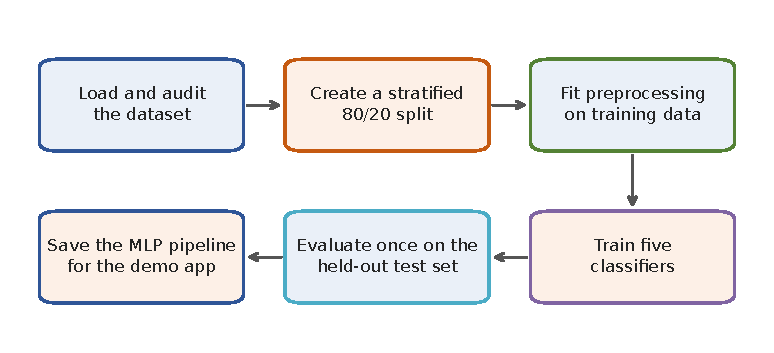
\includegraphics[width=\textwidth]{figures/workflow.pdf}
    \caption{Sequence of the experiment, from the initial data audit through preprocessing and evaluation to assembly of the application pipeline.}
    \label{fig:workflow}
\end{figure}

\subsection{Dataset description}\label{subsec:dataset}

The local CSV has 768 rows, with eight predictor columns and a target named \texttt{Outcome}. Of these records, 500 are labelled outcome 0 (65.10\%) and 268 are labelled outcome 1 (34.90\%). The audit found no exact duplicate rows. Table~\ref{tab:variables} defines the nine columns using descriptions from the Kaggle data card and the original study \cite{uciKagglePima,smith1988adap}.

\begin{table}[t]
\caption{Predictors and target recorded in the local Pima Indians Diabetes dataset.}\label{tab:variables}
\centering
\begin{tabular}{@{}p{0.31\textwidth}p{0.61\textwidth}@{}}
\toprule
Variable & Description \\
\midrule
Pregnancies & Recorded number of pregnancies \\
Glucose & Plasma glucose concentration measured two hours after an oral glucose tolerance test (mg/dL) \\
BloodPressure & Diastolic blood pressure measured in mmHg \\
SkinThickness & Triceps skin-fold thickness measured in mm \\
Insulin & Serum insulin measured after two hours ($\mu$U/mL) \\
BMI & Body mass index in $\mathrm{kg}/\mathrm{m}^{2}$ \\
DiabetesPedigreeFunction & Dataset-specific score representing family history \\
Age & Patient age in years \\
Outcome & Recorded outcome class: 0 for no diabetes and 1 for diabetes \\
\bottomrule
\end{tabular}
\end{table}

The Kaggle data card describes the participants as women of Pima Indian heritage who were at least 21 years old \cite{uciKagglePima}. This narrowly defined sample cannot represent the general population. Accordingly, references to ``diabetes'' in this report denote the value stored in \texttt{Outcome}, not a diagnosis produced by the software.

\subsection{Data audit and preprocessing}\label{subsec:preprocessing}

For this experiment, the preprocessing rule interprets zeros in five measurement columns as missing observations. Figure~\ref{fig:audit} presents the outcome distribution alongside the number of zeros in these columns. There are 374 rows with zero insulin and 227 with zero skin thickness; the corresponding counts for blood pressure, BMI, and glucose are 35, 11, and 5. The rule does not cover pregnancies or age, so zeros in those columns were left unchanged.

\begin{figure}[t]
    \centering
    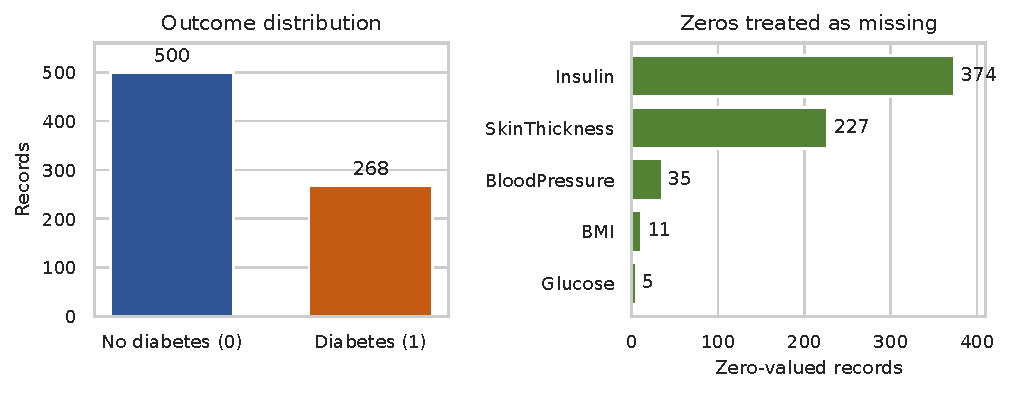
\includegraphics[width=\textwidth]{figures/dataset_audit.pdf}
    \caption{Outcome-class distribution and counts of zeros treated as missing in the five selected physiological measurements.}
    \label{fig:audit}
\end{figure}

We split the data before performing either imputation or scaling. Using a stratified 80/20 split with \texttt{random\_state=42} yielded 614 training rows and 154 test rows. The training portion comprises 400 negative and 214 positive examples, while the test portion comprises 100 negative and 54 positive examples.

Within the training set, each zero in the five selected columns was replaced with the non-zero median of that column. The resulting training medians were 117 for glucose, 72 for blood pressure, 29 for skin thickness, 125 for insulin, and 32.4 for BMI. These same fixed values were used to impute the test set. We fitted standard scaling after imputation, still using only the training data. Each feature $x_j$ was transformed as

\begin{equation}
z_j = \frac{x_j-\mu_j}{\sigma_j},
\label{eq:standardization}
\end{equation}

where $\mu_j$ and $\sigma_j$ denote the training-set mean and standard deviation. Scikit-learn pipelines and column transformations link these preprocessing operations into one sequence \cite{pedregosa2011scikit}. The same sequence is retained in the saved artifact, allowing the app to transform inputs exactly as they were transformed during training.

The correlation heatmap required a separate descriptive calculation. For this analysis, zeros in the same five features were marked as missing, and Pearson correlations were computed from the available value pairs. These calculations did not form part of the training pipeline.

\subsection{Software and reproducibility}\label{subsec:software}

We ran the experiment with Python 3.12, scikit-learn 1.9.0, pandas 2.3.3, NumPy 2.5.2, Matplotlib 3.11.1, and seaborn 0.13.2. The custom KNN relies directly on NumPy, while scikit-learn provides the other classifiers and evaluation measures \cite{pedregosa2011scikit}. Execution took place without GPU acceleration on an x86-64 computer equipped with a 13th-generation Intel Core i7-13620H processor and 31 GiB of memory.

The repository fixes the dependency versions and records both the random seed and model configurations. Running \texttt{generate\_figures.py} repeats the experiment and regenerates the numerical results, tables, and figures reported here. During the document build, automated checks compare the regenerated outputs with the values stated in the manuscript.

\section{MACHINE LEARNING CLASSIFIERS}\label{sec:models}

All five classifiers were trained with the fixed configurations shown in Table~\ref{tab:settings}. We used these settings without a grid search or another hyperparameter-search procedure.

\begin{table}[!htbp]
\caption{Fixed configuration of each classifier in the experiment.}\label{tab:settings}
\centering
\begin{tabular}{@{}p{0.25\textwidth}p{0.67\textwidth}@{}}
\toprule
Classifier & Configuration \\
\midrule
Custom KNN & $k=7$; Euclidean distance; unweighted majority voting \\
Decision Tree & Gini impurity; maximum depth 4; at least 10 samples required to split a node; seed 42 \\
Calibrated SVM & RBF kernel; $C=1$; $\gamma=\texttt{scale}$; sigmoid calibration with five folds; \texttt{ensemble=False} \\
Gaussian Naive Bayes & Default scikit-learn variance smoothing \\
MLP & Hidden layers (16, 8); ReLU activation; Adam optimizer; $\alpha=0.01$; maximum 1000 iterations; seed 42 \\
\bottomrule
\end{tabular}
\end{table}

\subsection{Custom \texorpdfstring{$k$}{k}-nearest neighbours}\label{subsec:knn}

The custom KNN classifier retained the standardized training rows and compared each new row with them. The Euclidean distance between a query vector $\mathbf{x}$ and a training vector $\mathbf{x}_i$ is

\begin{equation}
d(\mathbf{x},\mathbf{x}_i)=\sqrt{\sum_{j=1}^{8}(x_j-x_{ij})^2}.
\label{eq:distance}
\end{equation}

For each query, the implementation selected the seven nearest training rows and assigned the class chosen by majority vote. The class 1 score was the proportion of those seven neighbours labelled 1. Standardization prevented features with wider numerical ranges from dominating the distance calculation. This procedure follows the nearest-neighbour principle described by Cover and Hart \cite{cover1967nearest}.

\subsection{Decision tree}\label{subsec:tree}

The decision tree formed recursive, single-feature splits. It assessed each candidate split using Gini impurity,

\begin{equation}
G = 1-\sum_{c\in\{0,1\}}p_c^2,
\label{eq:gini}
\end{equation}

where $p_c$ denotes the proportion of class $c$ in a node. Tree depth was capped at 4, and a node required at least 10 samples before it could be split. These constraints were intended to limit model complexity and reduce overfitting. The classifier belongs to the classification-tree family described by Breiman et al. \cite{breiman1984cart}.

\subsection{Calibrated support vector machine}\label{subsec:svm}

The SVM was fitted with a radial basis function kernel,

\begin{equation}
K(\mathbf{x},\mathbf{x}')=\exp\left(-\gamma\lVert\mathbf{x}-\mathbf{x}'\rVert^2\right),
\label{eq:rbf}
\end{equation}

with $C=1$ and scikit-learn's \texttt{scale} setting for $\gamma$. This kernel allows a non-linear decision boundary in the transformed feature space. The method is based on the maximum-margin SVM developed by Cortes and Vapnik \cite{cortes1995svm}. Five-fold sigmoid calibration, configured with \texttt{ensemble=False}, supplied the scores used for the ROC curve. The experiment did not include a separate assessment of calibration error.

\subsection{Gaussian Naive Bayes}\label{subsec:nb}

Gaussian Naive Bayes represents each feature with a class-specific normal distribution and combines the resulting likelihoods through Bayes' rule. It assumes that the features are conditionally independent once the class is known. Clinical measurements are unlikely to satisfy this assumption exactly, but the classifier provides a computationally light baseline. We used the default scikit-learn configuration \cite{pedregosa2011scikit}.

\subsection{Multi-layer perceptron}\label{subsec:mlp}

The MLP had two hidden layers containing 16 and 8 units. Both layers used rectified linear unit activation, while Adam updated the network weights. A regularization value of $\alpha=0.01$ penalized large weights. Training used seed 42 and could run for no more than 1000 iterations. This architecture follows the layered learning and back-propagation approach described by Rumelhart et al. \cite{rumelhart1986backprop}.

The fitted MLP was stored in a single joblib pipeline with its imputer and scaler. When a user supplies the same eight features, the Streamlit interface runs the fitted preprocessing steps before showing the predicted class and score. The interface presents this output as a model estimate, not as medical advice.

\section{EVALUATION METRICS}\label{sec:metrics}

For the following definitions, true positives (TP) and true negatives (TN) are positive and negative rows classified correctly. A false positive (FP) is a negative row assigned to the positive class, whereas a false negative (FN) is a positive row assigned to the negative class. The threshold-based measures are

\begin{align}
\text{Accuracy} &= \frac{TP+TN}{TP+TN+FP+FN}, \label{eq:accuracy}\\
\text{Precision} &= \frac{TP}{TP+FP}, \label{eq:precision}\\
\text{Sensitivity} &= \frac{TP}{TP+FN}, \label{eq:sensitivity}\\
\text{Specificity} &= \frac{TN}{TN+FP}, \label{eq:specificity}\\
F_1 &= \frac{2\,\text{Precision}\,\text{Sensitivity}}
{\text{Precision}+\text{Sensitivity}}. \label{eq:f1}
\end{align}

Accuracy is the fraction of all rows classified correctly. Precision measures the correctness of positive predictions, and sensitivity measures the share of recorded positives that the classifier detects. Specificity gives the share of negatives correctly rejected. F1 combines precision and sensitivity through their harmonic mean.

The Matthews correlation coefficient (MCC) incorporates all four entries of the confusion matrix:

\begin{equation}
\mathrm{MCC}=\frac{TP\times TN-FP\times FN}
{\sqrt{(TP+FP)(TP+FN)(TN+FP)(TN+FN)}}.
\label{eq:mcc}
\end{equation}

Matthews introduced MCC \cite{matthews1975mcc}. It is informative when the class counts differ because a high score requires correct classification in both classes \cite{chicco2020mcc}. Values range from $-1$ to 1: 1 denotes perfect agreement, 0 indicates no correlation between predicted and observed labels, and $-1$ denotes complete disagreement.

A receiver operating characteristic (ROC) curve plots sensitivity against the false-positive rate as the score threshold changes \cite{fawcett2006roc}. Its area, ROC--AUC, is the probability that a randomly chosen positive row receives a higher score than a randomly chosen negative row \cite{hanley1982auc}. An AUC of 0.5 indicates chance-level ranking, whereas 1 indicates perfect ranking. This measure neither determines a clinical decision threshold nor demonstrates that the scores are well calibrated.

\section{RESULTS AND DISCUSSION}\label{sec:results}

\subsection{Exploratory observations}\label{subsec:eda}

Figure~\ref{fig:audit} shows a moderate imbalance toward outcome 0. Always predicting 0 would yield 65.10\% accuracy, yet it would leave every positive row undetected. We therefore consider sensitivity, F1, AUC, and MCC alongside accuracy.

For the descriptive analysis in Figure~\ref{fig:correlation}, the selected zero values were treated as missing before pairwise Pearson correlations were calculated. Glucose has the strongest linear association with Outcome ($r=0.49$). The next largest correlations are for BMI ($r=0.31$), insulin ($r=0.30$), skin thickness ($r=0.26$), and age ($r=0.24$). These sample correlations measure linear association, not causation.

\begin{figure}[t]
    \centering
    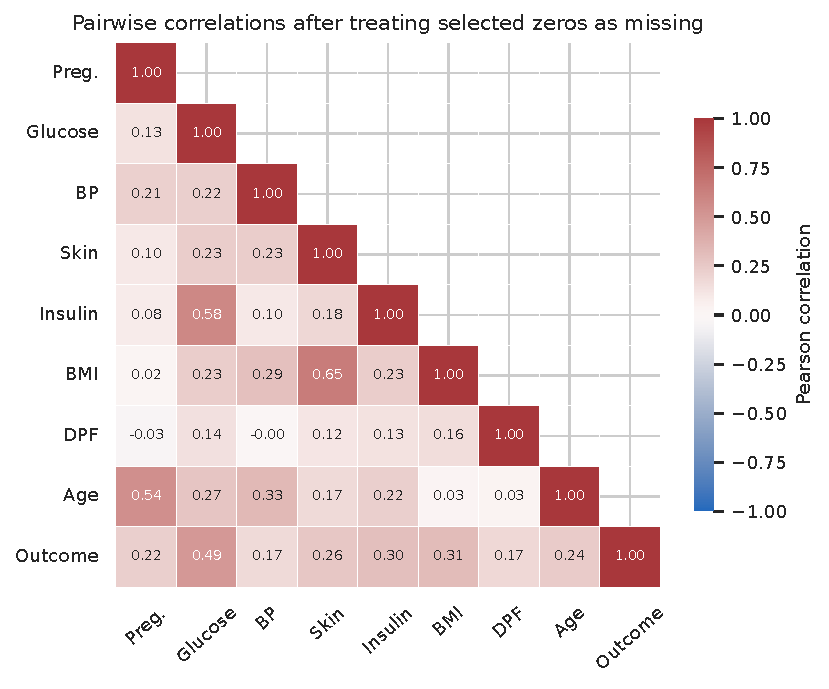
\includegraphics[width=0.88\textwidth]{figures/correlation_heatmap.pdf}
    \caption{Lower-triangle matrix of pairwise Pearson correlations. Selected zero values in the five measurement fields were treated as missing and excluded from the corresponding pairwise calculations.}
    \label{fig:correlation}
\end{figure}

\subsection{Model comparison}\label{subsec:comparison}

Table~\ref{tab:metrics} summarizes the complete held-out results. The decision tree leads in accuracy (78.57\%), precision (69.81\%), sensitivity (68.52\%), F1 (69.16\%), and MCC (0.527). Its specificity of 84.00\% matches that of the calibrated SVM, while the MLP records the highest ROC--AUC at 81.04\%.

\begin{table}[!htbp]
\caption{Classifier performance on the 154-row held-out test set. All measures except MCC are percentages. Bold type identifies the highest value in each column, with a tie for the best specificity.}\label{tab:metrics}
\centering
\footnotesize
\setlength{\tabcolsep}{2.5pt}
\begin{tabular}{@{}lrrrrrrr@{}}
\toprule
Model & Acc. & Prec. & Sens. & Spec. & F1 & ROC--AUC & MCC \\
\midrule
Custom KNN & 72.73\% & 62.50\% & 55.56\% & 82.00\% & 58.82\% & 79.00\% & 0.387 \\
Decision Tree & \textbf{78.57\%} & \textbf{69.81\%} & \textbf{68.52\%} & \textbf{84.00\%} & \textbf{69.16\%} & 78.87\% & \textbf{0.527} \\
Calibrated SVM & 74.03\% & 65.22\% & 55.56\% & \textbf{84.00\%} & 60.00\% & 79.63\% & 0.412 \\
Gaussian NB & 70.13\% & 56.67\% & 62.96\% & 74.00\% & 59.65\% & 76.46\% & 0.362 \\
MLP & 72.73\% & 61.54\% & 59.26\% & 80.00\% & 60.38\% & \textbf{81.04\%} & 0.396 \\
\bottomrule
\end{tabular}

\end{table}

\begin{figure}[t]
    \centering
    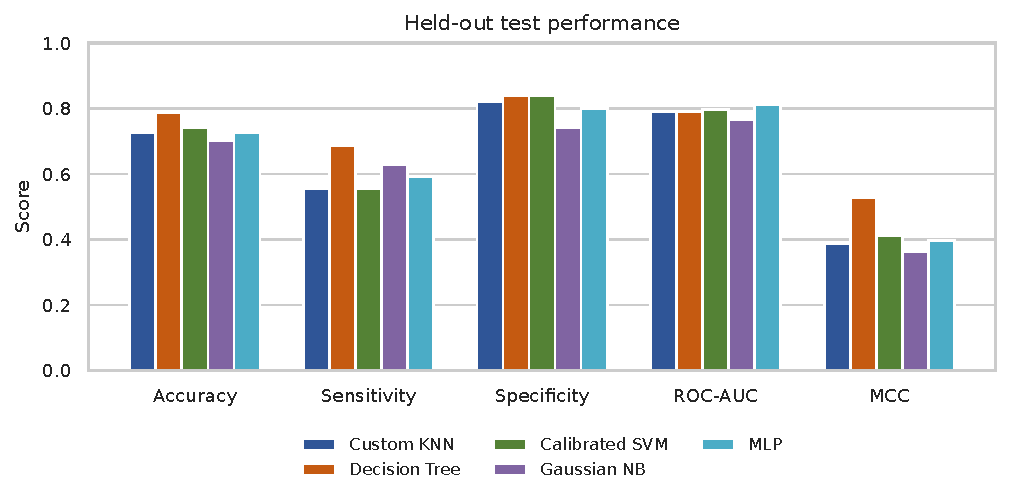
\includegraphics[width=\textwidth]{figures/model_comparison.pdf}
    \caption{Comparison of accuracy, class-specific measures, AUC, and MCC across the five classifiers.}
    \label{fig:comparison}
\end{figure}

The preferred model changes with the evaluation measure. The decision tree performs best on the threshold-based measures at the default classification threshold, whereas the MLP has the highest AUC across thresholds. Only 1.41 percentage points separate the MLP and calibrated SVM AUC values. Because these results come from a single split without repeated cross-validation or a significance test, the measured difference does not establish that the MLP is superior.

\subsection{Error patterns}\label{subsec:errors}

The confusion matrices in Figure~\ref{fig:confusion} make the error patterns explicit. The decision tree correctly labels 84 of the 100 negative rows and 37 of the 54 positive rows, leaving 16 false positives and 17 false negatives. KNN and the calibrated SVM each identify 30 positives and miss 24. Gaussian Naive Bayes identifies 34 positives but also generates 26 false positives; consequently, its sensitivity is higher than that of KNN and SVM, but its specificity is lower. The MLP falls between these patterns, producing 32 true positives, 22 false negatives, 80 true negatives, and 20 false positives.

\begin{figure}[t]
    \centering
    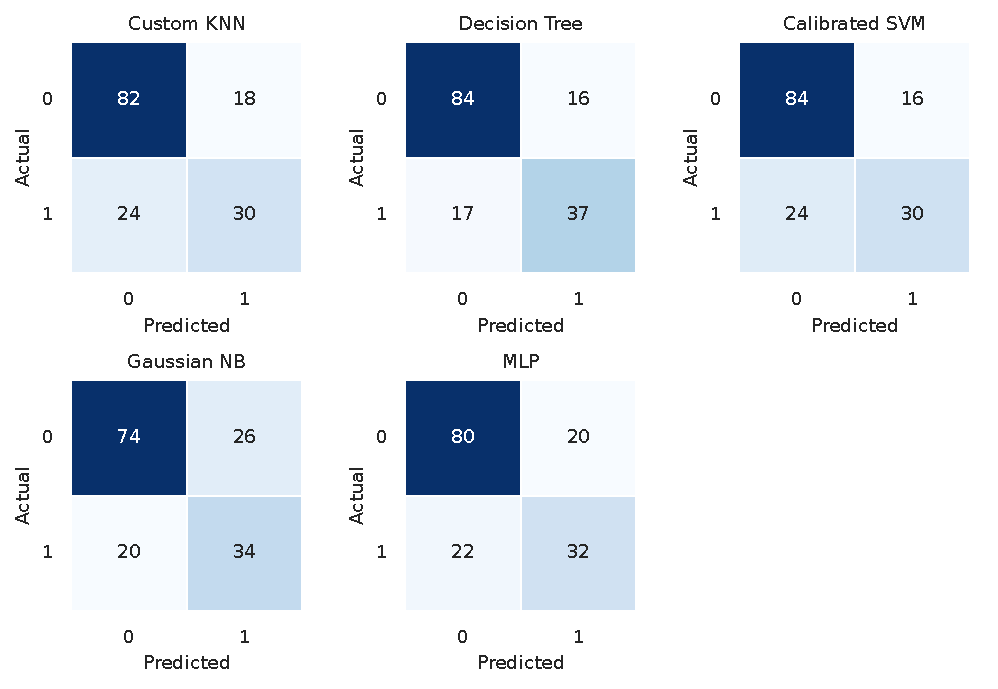
\includegraphics[width=\textwidth]{figures/confusion_matrices.pdf}
    \caption{Held-out confusion matrices for all five classifiers, with actual labels in rows and predicted labels in columns.}
    \label{fig:confusion}
\end{figure}

In practice, false negatives and false positives need not have equal consequences. No error costs or clinical operating threshold were specified in this experiment; the confusion matrices therefore support only a comparison of model error patterns.

\subsection{ROC analysis}\label{subsec:roc}

For most thresholds, every ROC curve in Figure~\ref{fig:roc} lies above the chance diagonal. The measured areas rank the MLP first, followed by the calibrated SVM, KNN, decision tree, and Gaussian Naive Bayes. This order is different from the accuracy ranking because AUC evaluates score ordering across thresholds, whereas accuracy is calculated from a single set of predicted labels.

\begin{figure}[t]
    \centering
    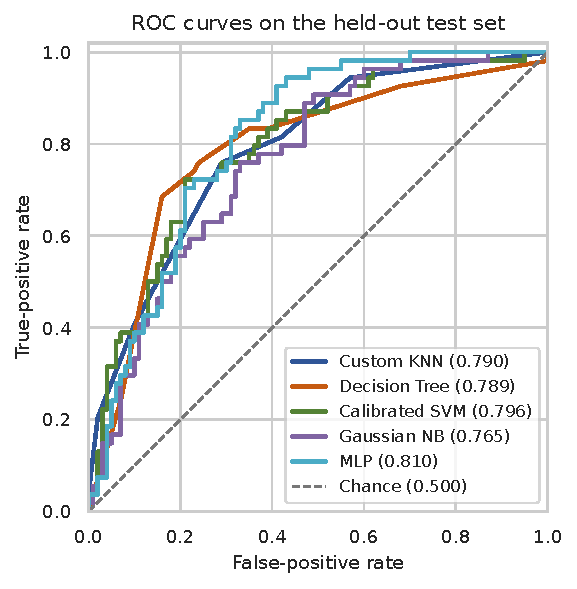
\includegraphics[width=0.84\textwidth]{figures/roc_curves.pdf}
    \caption{ROC curves with AUC values for the held-out test set; the diagonal denotes chance-level ranking.}
    \label{fig:roc}
\end{figure}

\subsection{Exploratory feature sensitivity}\label{subsec:importance}

We estimated permutation importance for the fitted MLP pipeline from the reproducible report run. Each raw test feature was shuffled separately 30 times, and the resulting change in ROC--AUC was recorded. Shuffling glucose produced the largest mean decrease on this test set (0.117), followed by age (0.053). BMI and insulin produced smaller positive changes, whereas the values for blood pressure and skin thickness remained close to zero.

\begin{figure}[!htbp]
    \centering
    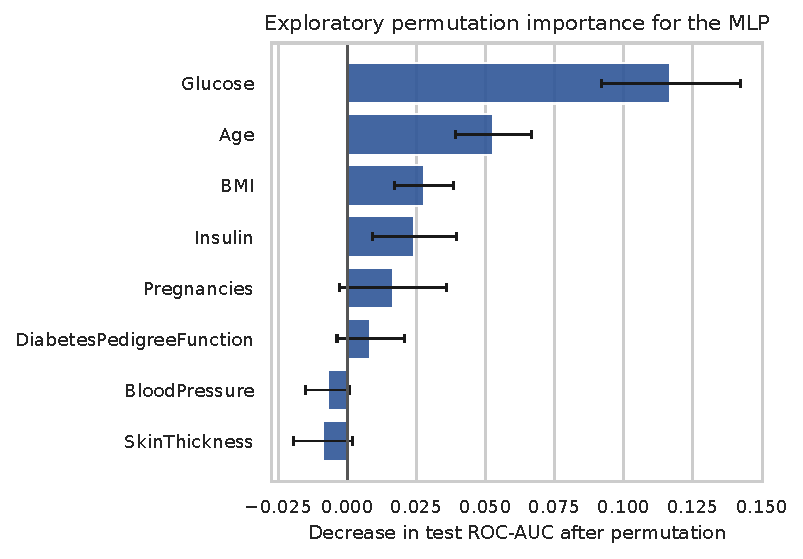
\includegraphics[width=0.88\textwidth]{figures/permutation_importance.pdf}
    \caption{Exploratory permutation importance for the MLP, estimated from 30 shuffles of each feature. Error bars represent one standard deviation across shuffles; sampling variation can produce negative values.}
    \label{fig:importance}
\end{figure}

These permutation scores are descriptive and do not support causal interpretation. Correlated predictors can share importance, and estimates from 154 test records may vary substantially. Model tuning did not use these values.

\subsection{Deployment demonstration}\label{subsec:deployment}

The Streamlit application loads the MLP pipeline from \path{out/models/diabetes_pipeline.joblib} because the MLP recorded the highest AUC in the comparison. The artifact contains the imputer, scaler, column order, and model together, so application inputs undergo the same preprocessing as the training data.

Because the MLP was chosen after inspection of the test results, the application cannot serve as an independent validation. Its output is neither an externally calibrated estimate of patient risk nor suitable evidence for diagnosis, screening, or treatment decisions.

\subsection{Limitations}\label{subsec:limitations}

The following limitations define how the results should be interpreted:

\begin{itemize}
    \item The small dataset covers only women of Pima Indian heritage who are at least 21 years old. Results in other populations may not match the performance measured here.
    \item Evaluation used one train--test split with stratification; it includes no repeated validation, uncertainty intervals, or external test data.
    \item All classifiers use fixed settings, and no documented hyperparameter search was conducted. In addition, the MLP was chosen for the application after its test results were available.
    \item Zero entries in five measurement columns are treated as missing. Because the Kaggle data card does not account for these zeros, this treatment is a modelling choice rather than a verified characteristic of every affected record. Median imputation cannot restore the original measurements and may conceal structure in the missingness.
    \item The positive class has fewer records, but the experiment applies neither class weighting nor threshold optimization.
    \item The project does not include clinical calibration, subgroup analysis, prospective testing, or external validation.
\end{itemize}

\FloatBarrier
\section{CONCLUSION}\label{sec:conclusion}

We compared five classifiers under the same preprocessing workflow, with every fitted preprocessing step restricted to the training data. On the held-out test set, the decision tree achieved the highest accuracy, sensitivity, F1, and MCC; the MLP achieved the highest ROC--AUC. These different rankings show that accuracy alone does not provide enough evidence for model selection. The confusion matrices further reveal how each classifier balances missed positives against false alarms.

The resulting workflow provides a reproducible five-model comparison and connects the saved MLP pipeline to a working Streamlit interface. Its findings are limited to this dataset and fixed split, and they do not establish a clinically valid predictor of diabetes. The application is therefore an educational demonstration of the implemented machine learning workflow.

\backmatter

\clearpage
\phantomsection
\addcontentsline{toc}{section}{REFERENCES}
\bibliography{references}

\end{document}
